\documentclass[12pt, a4paper, oneside]{ctexart}
\usepackage{amsmath, amsthm, amssymb, bm, color, graphicx, geometry, mathrsfs,extarrows, braket, booktabs, array, xcolor, fontspec, appendix, float, subfigure, wrapfig}
\usepackage[colorlinks,linkcolor=red,anchorcolor=blue,citecolor=blue,urlcolor=blue,menucolor=black]{hyperref}

%%%% 设置中文字体 %%%%
\setCJKmainfont{方正新书宋_GBK.ttf}[ BoldFont = 方正小标宋_GBK, ItalicFont = 方正楷体_GBK]
%%%% 设置英文字体 %%%%
\setmainfont{Times New Roman}
\setsansfont{Calibri}
\setmonofont{Consolas}

%%%% 设置代码块 %%%%
% 在vscode中使用minted需要先配置python解释器, Ctrl+Shift+P, 输入Python: Select Interpreter选择安装了Pygments的Python版本. 再在setting.json中xelatex和pdflatex的参数中加入 "--shell-escape", 即可
% TeXworks中配置方法参考: https://blog.csdn.net/RobertChenGuangzhi/article/details/108140093
\usepackage{minted}
\renewcommand{\theFancyVerbLine}{
    \sffamily\textcolor[rgb]{0.5,0.5,0.5}{\scriptsize\arabic{FancyVerbLine}}} % 修改代码前序号大小
\newmintinline{cpp}{linenos, breaklines, frame=lines}  % 使用\cppinline{代码}
\newminted{cpp}{linenos, breaklines, frame=lines}  % 使用\begin{cppcode}代码\end{cppcode}
\newmintinline{python}{linenos, breaklines, frame=lines, python3}  % 使用\pythoninline{代码}
\newminted{python}{linenos, breaklines, frame=lines, python3}  % 使用\begin{pythoncode}代码\end{pythoncode}
\newmintedfile{python}{linenos, breaklines, frame=lines, python3}  % 使用\pythonfile{代码地址}

%%%% 设置行间距与页边距 %%%%
\linespread{1.2}
\geometry{left=2.5cm, right=2.5cm, top=2.5cm, bottom=2.5cm}

%%%% 定理类环境的定义 %%%%
\newtheorem{example}{例}            % 整体编号
\newtheorem{theorem}{定理}[section] % 定理按section编号
\newtheorem{definition}{定义}
\newtheorem{axiom}{公理}
\newtheorem{property}{性质}
\newtheorem{proposition}{命题}
\newtheorem{lemma}{引理}
\newtheorem{corollary}{推论}
\newtheorem{remark}{注解}
\newtheorem{condition}{条件}
\newtheorem{conclusion}{结论}
\newtheorem{assumption}{假设}
\numberwithin{equation}{section}  % 公式按section编号 (公式右端的小括号)
\newtheorem{algorithm}{算法}
\newsavebox{\nameinfo}
\renewenvironment{title}[1]{
    \sbox{\nameinfo}{\zihao{4} #1}
    \begin{center}
    \zihao{-2}\bf
}{\vspace{-0.2cm}\\\usebox{\nameinfo}\end{center}}  % \begin{title}{作者信息}

%%%% 图片相对路径 %%%%
\graphicspath{{figure/}} % 当前目录下的figure文件夹, {../figure/}则是父目录的figure文件夹
\setlength{\abovecaptionskip}{-0.2cm}  % 缩紧图片标题与图片之间的距离
\setlength{\belowcaptionskip}{0pt} 

\everymath{\displaystyle} % 默认全部行间公式, 想要变回行内公式使用\textstyle
\DeclareMathOperator*\uplim{\overline{lim}}     % 定义上极限 \uplim_{}
\DeclareMathOperator*\lowlim{\underline{lim}}   % 定义下极限 \lowlim_{}
\DeclareMathOperator*{\argmax}{arg\,max}  % \argmin
\DeclareMathOperator*{\argmin}{arg\,min}  % \argmax
\let\leq=\leqslant % 简写小于等于\leq (将全部leq变为leqslant)
\let\geq=\geqslant % 简写大于等于\geq (将全部geq变为geqslant)

%%%% 一些宏定义 %%%%%
\def\bd{\boldsymbol}        % 加粗(向量) boldsymbol
\def\disp{\displaystyle}    % 使用行间公式 displaystyle(默认)
\def\tsty{\textstyle}       % 使用行内公式 textstyle
\def\sign{\text{sign}}      % sign function
\def\wtd{\widetilde}        % 宽波浪线 widetilde
\def\R{\mathbb{R}}          % Real number
\def\C{\mathbb{C}}          % Complex number
\def\Q{\mathbb{Q}}          % Rational number
\def\N{\mathbb{N}}          % Natural number
\def\d{\mathrm{d}}          % differential operator
\def\e{\mathrm{e}}          % Euler's number
\def\i{\mathrm{i}}          % imaginary number
\def\re{\mathrm{Re}}        % Real part
\def\im{\mathrm{Im}}        % Imaginary part
\def\L{\mathcal{L}}         % Loss function
\def\wdh{\widehat}          % 宽帽子 widehat
\def\ol{\overline}          % 上横线 overline
\def\ul{\underline}         % 下横线 underline
\def\add{\vspace{1ex}}      % 增加行间距
\def\del{\vspace{-1.5ex}}   % 减少行间距

%%%% 正文开始 %%%%
\begin{document}
\begin{title}{强基数学002\quad 吴天阳\quad 2204210460}
    CVPR第二次作业
\end{title}
\setcounter{section}{1}
\subsection{图像参数化几何变换原理}
1. 平移变换(自由度为$2$)
\begin{equation*}
    \bd{x}' = \bd{x}+\bd{t}\iff \bd{x}' = \left[\begin{matrix}
        1&0&t_1\\ 0&1&t_2\\ 0&0&1
    \end{matrix}\right]\left[\begin{matrix}
        x_1\\x_2\\1
    \end{matrix}\right]
\end{equation*}

2. 旋转变换(自由度为$1$)
\begin{equation*}
    \bd{x}' = R_{\theta}\bd{x}\iff \bd{x}' = \left[\begin{matrix}
        \cos\theta&-\sin\theta&0\\
        \sin\theta&\cos\theta&0\\
        0&0&1
    \end{matrix}\right]\left[\begin{matrix}
        x_1\\x_2\\1
    \end{matrix}\right]
\end{equation*}

3. 欧式变化(自由度为$3$)
\begin{equation*}
    \bd{x}' = [R_\theta|\bd{t}]\bd{x}\iff \bd{x}' = \left[\begin{matrix}
        \cos\theta&-\sin\theta&t_1\\
        \sin\theta&\cos\theta&t_2\\
        0&0&1
    \end{matrix}\right]\left[\begin{matrix}
        x_1\\x_2\\1
    \end{matrix}\right]
\end{equation*}

4. 相似变换(自由度为$4$)
\begin{equation*}
    \bd{x}' = [R_\theta|\bd{t}]\bd{x}\iff \bd{x}' = \left[\begin{matrix}
        s\cdot \cos\theta&-s\cdot\sin\theta&t_1\\
        s\cdot \sin\theta&s\cdot \cos\theta&t_2\\
        0&0&1
    \end{matrix}\right]\left[\begin{matrix}
        x_1\\x_2\\1
    \end{matrix}\right]
\end{equation*}

5. 放射变换(自由度为$6$)
\begin{equation*}
    \bd{x}' = \bd{x}+\bd{t}\iff \bd{x}' = \left[\begin{matrix}
        a_{11}&a_{12}&t_1\\
        a_{21}&a_{22}&t_2\\
        0&0&1
    \end{matrix}\right]\left[\begin{matrix}
        x_1\\x_2\\1
    \end{matrix}\right]
\end{equation*}
\subsection{前向变换与逆向变换}
设变换矩阵为$T$,原图像记为$f(\cdot)$,变换后的图像记为$g(\cdot)$,则有
\begin{equation*}
    g(T\bd{x}) = f(\bd{x}),\qquad g(\bd{x}) = f(T^{-1}\bd{x}).
\end{equation*}
其中,前者为前向变换(forward warping),后者为逆向变换(inverse warping). 

前向变换中,由于$\bd{x}$的参数为整数,而$T\bd{x}$不一定为整数,所以填充时会出现空缺部分;而逆向变换中,计算$T^{-1}\bd{x}$非整数时,可通过像素插值算法获得该像素处的近似值,可以很好解决空缺问题.
\subsection{下抽样原理与内插方法原理}
\subsubsection{采样定理}
下抽样原理即采样定理. 下面定理描述的是对一维信号进行采样的结论,可类比得到二维图像的采样结论.
\begin{theorem}[Shannon-Nyquist定理,采样定理]
    设采样频率为$f_s$,信号中最大频率为$f_{max}$,当$f_x > 2f_{max}$时,采样后的信息完整保留了原始信号的信息,也即可通过采样信息复原出原始信号. (实际引用中一般取采样频率为最大频率的$2.56\sim 4$倍)
\end{theorem}
\begin{proof}
    考虑对原信号做基数为$N$的离散Fourier级数展开,将一组Fourier基记为(即对复平面单位圆做$N$等分)
    \begin{equation*}
     B_k(x) = \e^{\frac{2\pi\i kx}{N}} = \e\left(\frac{kx}{N}\right),\quad (0\leq k\leq N-1)   
    \end{equation*}
    其中$\e(x) = \e^{2\pi ix}$. 于是原始信号可表示为
    \begin{equation*}
        g(x) = \sum_{k=0}^{N-1}c_kB_k(x).
    \end{equation*}
    其中$c_k$可通过对原信号进行快速Fourier变换得到.\add

    \textbf{注}:由Euler公式可知,$B_k(x) = \cos(\frac{2\pi kx}{N}) + \i \sin(\frac{2\pi kx}{N})$,\add 所以$B_k$在原信号中对应的频率为$\frac{k}{N}$. 由于单位圆具有对称性,$\forall 0\leq k\leq \lfloor\frac{N-1}{2}\rfloor$有$B_{N-k} = B_{-k}$,\add 所以$B_k$与$B_{N-k}$具有相同的频率. 这说明,如果$f$为Fourier级数中最大的频率,则频域图的周期为$2f$.

    假设采样周期为$P$,则采样频率为$f_s = \frac{1}{P}$,则有
    \begin{equation*}
        B_{k+\frac{N}{P}}(nP) = \e\left(\frac{(k+\frac{N}{P})nP}{N}\right) = \e\left(\frac{knP}{N}+n\right)=\e\left(\frac{knP}{N}\right) = B_k(nP),\quad(n=1,2,\cdots)
    \end{equation*}
    上式说明,若原信号中同时存在频率为$\frac{k}{N}$与$\frac{k}{N}+\frac{1}{P}$的信号,\add 则它们会在$P,2P,\cdots, nP$处取值相同,则无法通过采样信息将这两种频率的区分开,所以只需保证这两种频率的信号不同时出现在原信号中即可.

    设$f_{max}$为原信号中的最大频率,且能通过Fourier级数表出,由上述的注释可知,频域的周期为$2f_{max}$,所以
    \begin{equation*}
        \frac{k}{N}+\frac{1}{P} - \frac{k}{N} > 2f_{max}\Rightarrow f_s > 2f_{max}.
    \end{equation*}
\end{proof}
\subsubsection{内插方法原理}
内插方法:设原图像大小为$N\times M$,记为$f(x,y),\ x\in[1,N],y\in[1,M]$,考虑二维平面中非整数点$(x^*, y^*)$,一种求解$f(x^*,y^*)$的方法.(也即将$f$延拓到$\R^2$中)

\textbf{近邻插值}:使用原图中距离$(x^*,y^*)$最近的像素进行代换. 记\del
\begin{equation*}
 (x_0,y_0) = \argmin_{(x,y)\in[1,N]\times[1,M]\cap \N^2}||(x,y)-(x^*,y^*)||_2,
\end{equation*}
其中$||\cdot||_2$表示2-范数,则$f(x^*,y^*) = f(x_0,y_0)$.

\textbf{双线性插值}:将$(x^*,y^*)$与周围整数点所围成的面积反比作为整数点对应像素的加权值,设$O(x^*,y^*)$周围存在四个整数点$A(x_h, y_h),\ B(x_h, y_l),\ C(x_l, y_l),\ D(x_l, y_h)$,对应的面积分别为$S_A = S(O,C),\ S_B = S(O, D),\ S_C = S(O, A),\ S_D = S(O, B)$,其中$S(O,A)$表示由点$O,A$所围成的面积,参考图\ref{双线性插值}. 则有\del\del

{\begin{wrapfigure}[10]{r}{.3\linewidth} % 文字环绕行数为13行, 图片靠右 (l为靠左), 图片占0.5的行宽
    \centering
    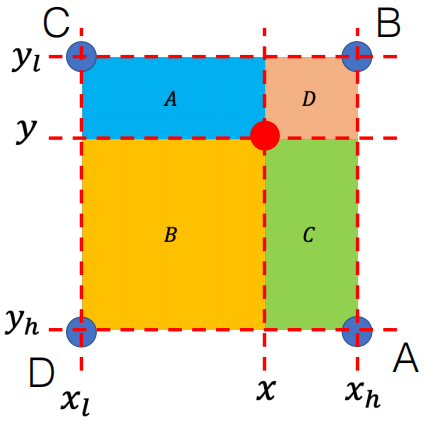
\includegraphics[scale=1.2]{双线性插值.png}
    \caption{双线性插值}
    \label{双线性插值}
\end{wrapfigure}
\begin{equation*}
    f(x^*, y^*) = S_Af(A)+S_Bf(B)+S_Cf(C)+S_Df(D).
\end{equation*}}
\vspace{2cm}\subsection{几何变换实验}
\end{document}
\begin{equation*}
    
\end{equation*}

\iffalse
%%%% 表格模板 %%%%
\renewcommand\arraystretch{0.8} % 设置表格高度为原来的0.8倍
\begin{table}[!htbp] % table标准
    \centering % 表格居中
    \begin{tabular}{p{1cm}<{\centering}p{1cm}<{\centering}p{3cm}<{\centering}p{5cm}<{\centering}} % 设置表格宽度
    %\begin{tabular}{cccc}
        \toprule
        $x_i$ & $f[x_1]$ & $f[x_i, x_{i+1}]$ & $f[x_i, x_{i+1}, x_{i+2}]$ \\
        \midrule
        $x_0$ & $f(x_0)$ &                  &                          \\
        $x_0$ & $f(x_0)$ & $f'(x_0)$        &                          \\
        $x_0$ & $f(x_1)$ & $\frac{f(x_1)-f(x_0)}{x_1-x_0}$ & $\frac{f(x_1)-f(x_0)}{(x_1-x_0)^2}-\frac{f'(x_0)}{x_1-x_0}$\\
        \bottomrule
    \end{tabular}
\end{table}

%%%% 文字环绕图片, 标题加注释 %%%%
{ % 一般将文字环绕部分的图和文字, 用大括号括起来, 避免对文字外的格式发生影响
\begin{wrapfigure}[13]{r}{.5\linewidth} % 文字环绕行数为13行, 图片靠右 (l为靠左), 图片占0.5的行宽
    \centering
    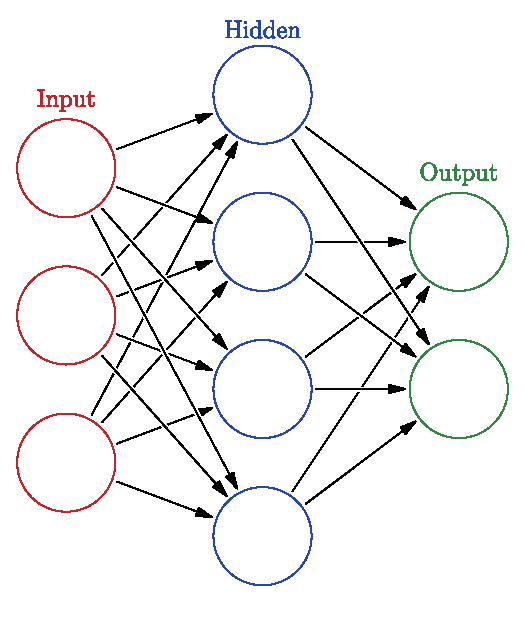
\includegraphics[scale=0.7]{neural_network.eps} % scale=0.7按比例缩放70%
    \caption{神经网络结构\protect\footnotemark[1]} % 记得加\protect, 设置1号脚标
    \label{figure-神经网络结构}
\end{wrapfigure}
\footnotetext[1]{图片来源: \url{https://en.wikipedia.org/wiki/File:Colored_neural_network.svg}}
文字文字
}

%%%% 普通图片, 标题加注释 %%%%
\begin{figure}[htbp] % h: 当前位置, t: 顶部, b: 底部, p: 浮动页, 这样组合指的是使用这个顺序进行排版
    \centering
    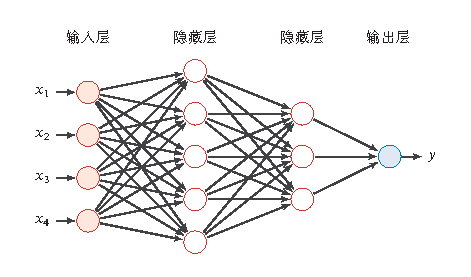
\includegraphics[scale=0.5]{前馈神经网络.eps}
    \caption{前馈神经网络\protect\footnotemark[1]}
    \label{figue-前馈神经网络}
\end{figure}
\footnotetext[1]{图片来源: 邱锡鹏, 神经网络与深度学习 \cite{ref-qxp}, 第92页}

%%%% 多组图 %%%%
    \begin{figure}[htbp]
        \centering
        \subfigure[迭代1次]  % 子图的标题
        {
            % 如果一行放三个图改成0.3\linewidth即可
            \begin{minipage}[b]{.45\linewidth}  % 0.45排版行距, 即一行放2个图, 一行放不下就换行
                \centering
                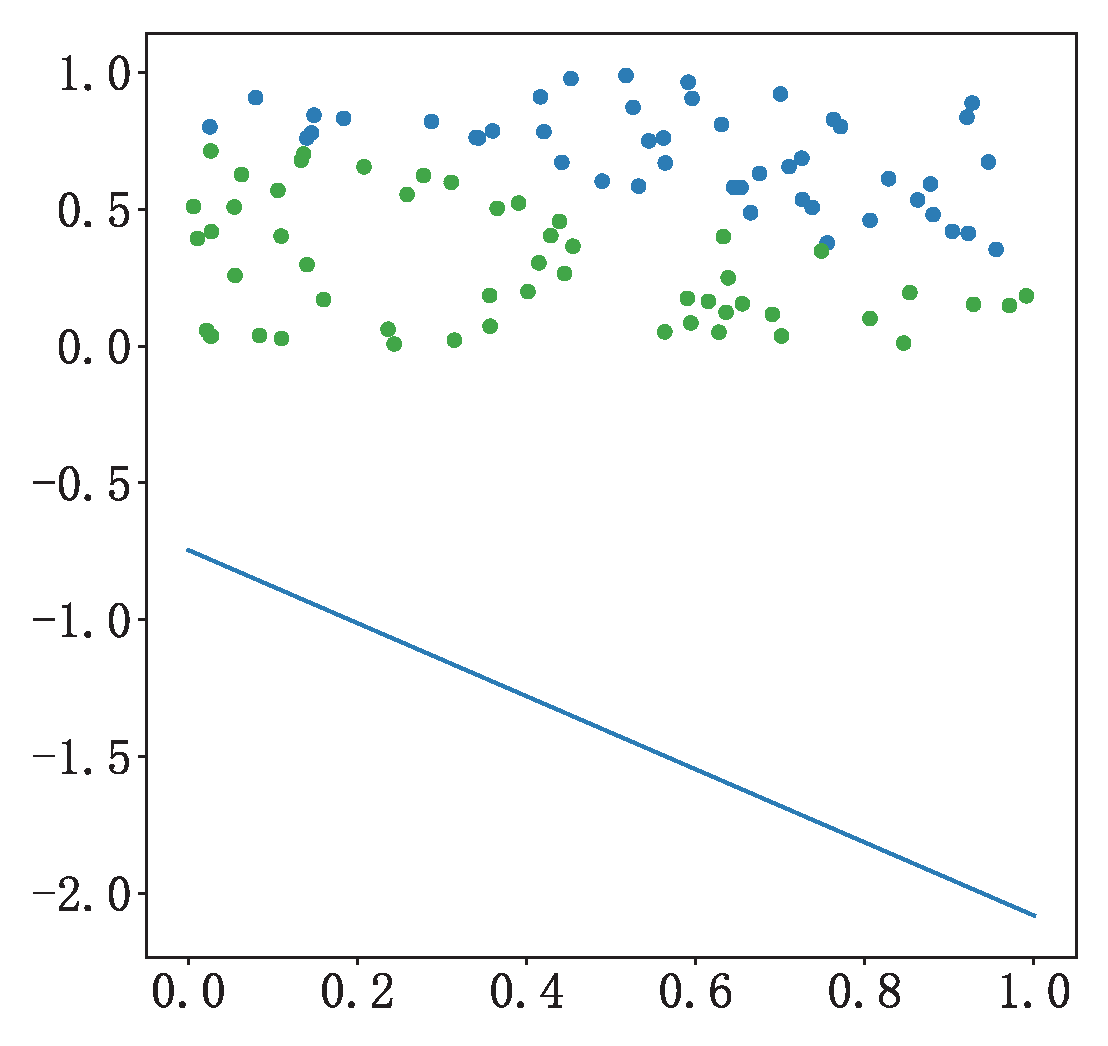
\includegraphics[scale=0.35]{1.eps}
            \end{minipage}
        }
        \subfigure[迭代100次]
        {
            \begin{minipage}[b]{.45\linewidth}
                \centering
                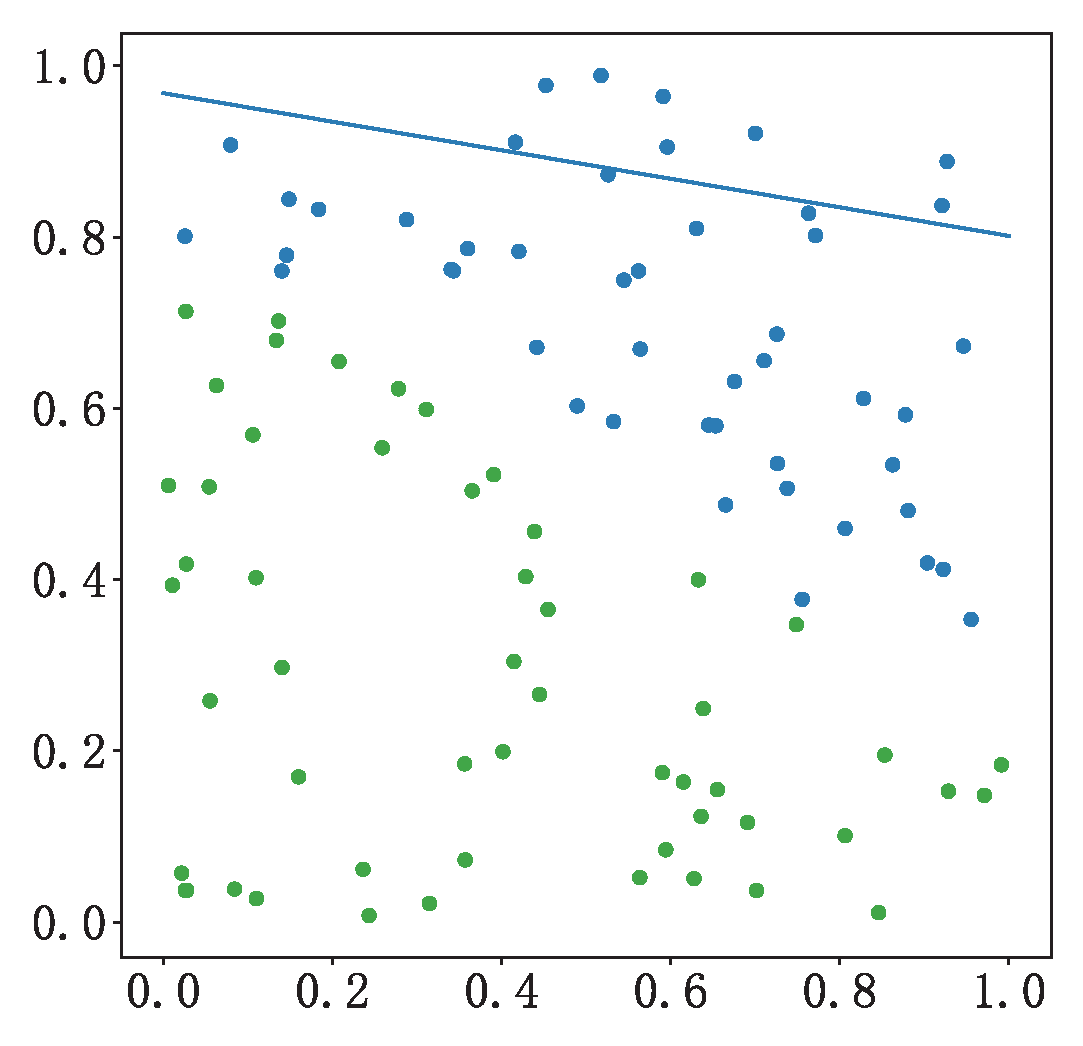
\includegraphics[scale=0.35]{100.eps}
            \end{minipage}
        }
        \subfigure[迭代500次]
        {
            \begin{minipage}[b]{.45\linewidth}
                \centering
                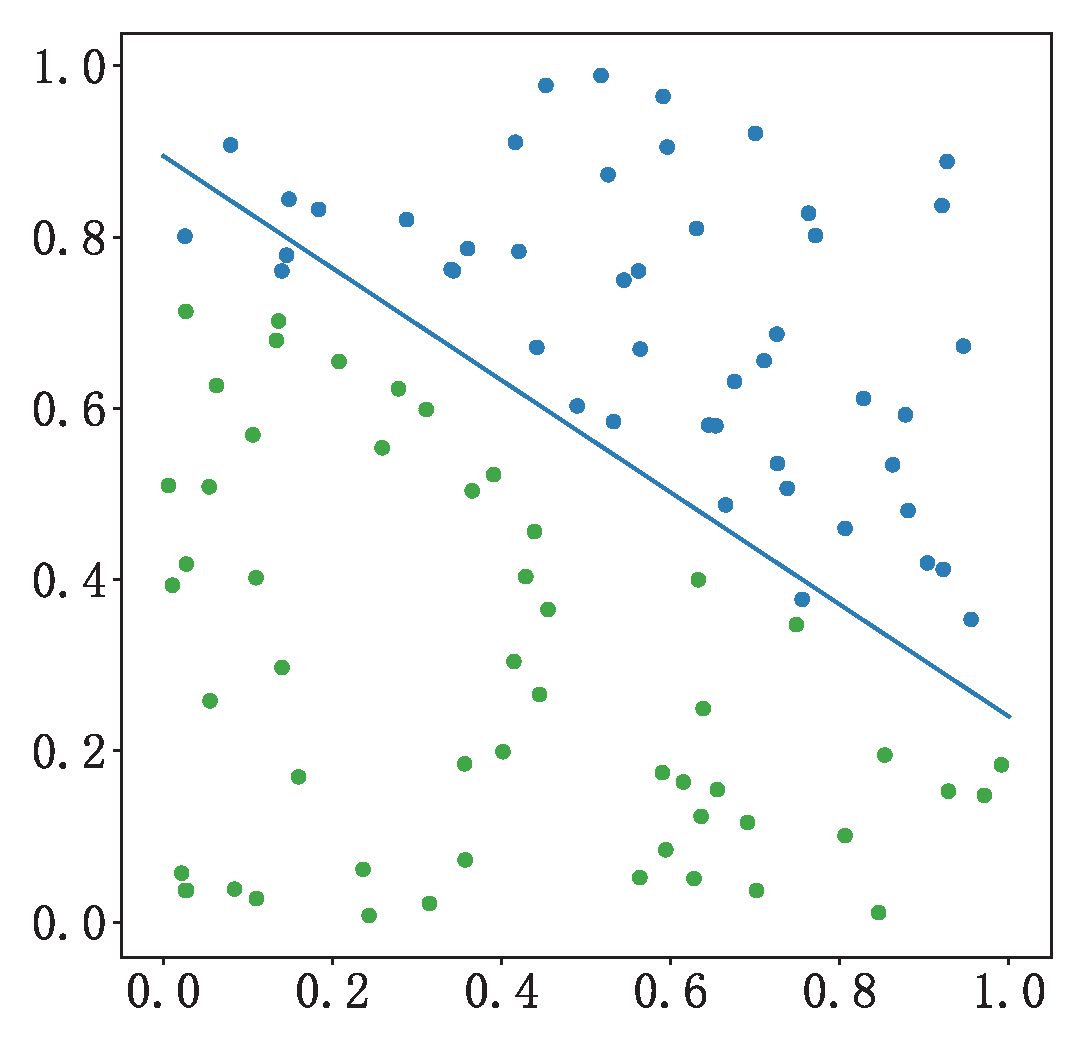
\includegraphics[scale=0.35]{500.eps}
            \end{minipage}
        }
        \subfigure[迭代2000次]
        {
            \begin{minipage}[b]{.45\linewidth}
                \centering
                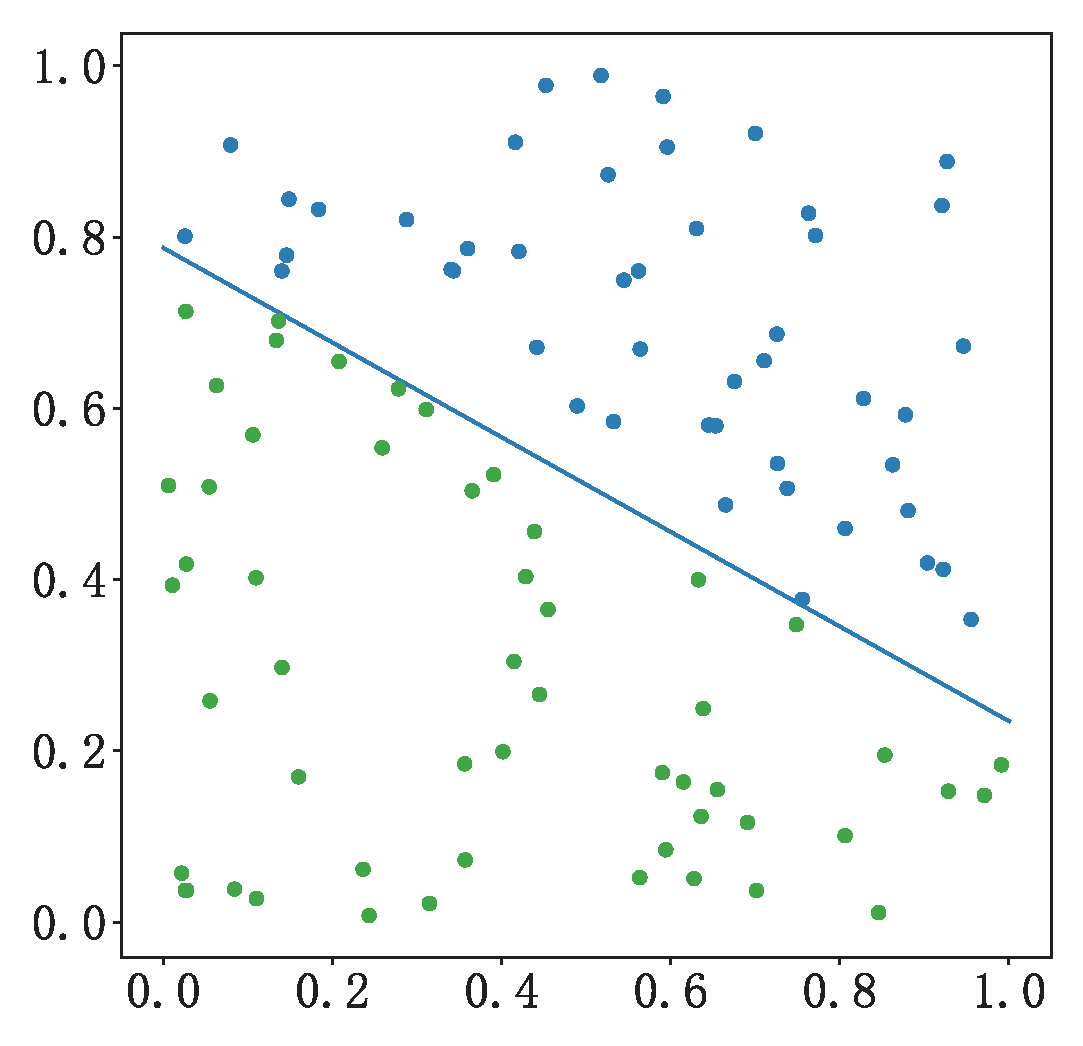
\includegraphics[scale=0.35]{2000.eps}
            \end{minipage}
        }
        \caption{迭代过程图}
        \label{figure-迭代过程图}
    \end{figure}
\fi
